\section{Problem Description}
\label{sec:ProblemDescription}

We present the problem of  testing \emph{model transformations}. A model transformation $MT(I,O)$ is a program applied on a set of input models $I$ to produce a set of output models $O$ as illustrated in Figure \ref{fig:exampleAndMT}. The set of all input models is specified by a metamodel $MM_{I}$ (For example, simplified {\UMLCD} in Figure \ref{fig:umlcd}). The set of all output models is specified by metamodel $MM_{O}$. The pre-condition of the model transformation $pre(MT)$ further constrains the input domain. A post-condition $post(MT)$ constrains the model transformation to producing a subset of all possible output models. The model transformation is developed based on a set of textual specification of requirements $MT_{Requirements}$.

\begin{figure} [!t]
\begin{center}

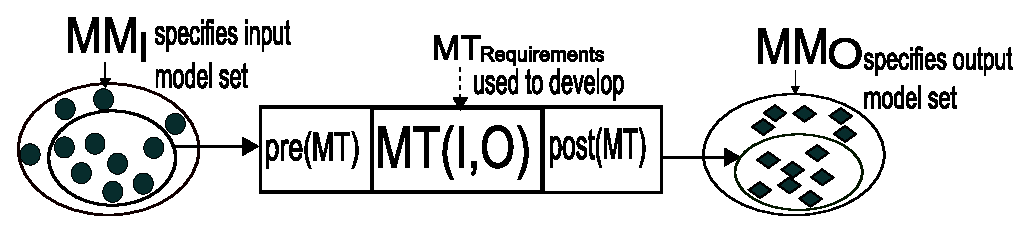
\includegraphics[width=3.5 in]{./figures/modelTransformation.eps}
\end{center}

\caption{A Model Transformation}
\label{fig:exampleAndMT}

\end{figure}

Automatic model generation for testing involves finding valid input models we call \emph{test models} from the set of all input models $I$. Test models must  satisfy constraints that increase the trust in the quality of these models as test data and thus should increase their capabilities to detect bugs in the model transformation $MT(I,O)$. Bugs may also exist in the input metamodel and its invariants $MM_{I}$ or the transformation pre-condition $pre(MT)$. However, in this paper we only focus on generating input models that can detect bugs in a transformation. In the process, we also generate input models that cannot be processed by a transformation (as they were unforeseen in $MT_{Requirements}$) which are then used to specify new pre-conditions.

\subsection{Transformation Case Study}

Our case study is the transformation from simplified {\UML} Class Diagram models to {\RDBMS} models called {\transfo}.  In this section we briefly describe {\transfo} and discuss why it is a representative transformation to validate test model generation strategies.

In testing we need input models that conform to the input metamodel $MM_{I}$ and transformation pre-condition $pre(MT)$. Therefore, we only discuss the $MM_{I}$ and $pre(MT)$ for {\transfo} and avoid discussion of the model transformation output domain. In Figure \ref{fig:umlcd}, we present the simplified {\UMLCD} input metamodel for {\transfo}. The concepts and relationships in the input metamodel are stored as an {\ecore} model \cite{emf2004} (Figure \ref{fig:umlcd} (a)). The invariants on the simplified {\UMLCD} {\ecore} model, expressed in {\textOCL} ({\OCL}) \cite{OCL}, are shown in Figure \ref{fig:umlcd} (b). The {\ecore} model and the invariants together represent the input domain for {\transfo}. The {\OCL} and {\ecore} are industry standards used to develop metamodels and specify different invariants on them. {\OCL} is not a domain-specific language to specify invariants. However, it is designed to formally encode natural language requirements specifications independent of its domain. 
%In \cite{oclShort} the authors present some limitations of {\OCL}.

The input metamodel $MM_{I}$ gives an initial specification of the input domain. However, the model transformation itself has a pre-condition $pre(MT)$ that test models need to satisfy to be correctly processed. Constraints in the pre-condition for {\transfo} include: (a) All {\Class} objects must have at least one primary {\Property} object (b) The type of an {\Property} object can be a {\Class} C, but finally the transitive closure of the type of {\Property} objects of {\Class} C must end with type {\PrimitiveDataType}. In our case we approximate this recursive closure constraint by stating that {\Property} object can be of type {\Class} up to a depth of 3 and the 4th time it should have a type {\PrimitiveDataType}. This is a finitization operation to avoid navigation in an infinite loop. (c) A {\Class} object cannot have an {\Association} and an {\Property} object of the same name (d) There are no cycles between non-persistent {\Class} objects.

We choose {\transfo} as our representative case study to validate input selection strategies. It serves as a sufficient case study for several reasons. The transformation is the benchmark proposed in the MTIP workshop at the MoDELS 2005 conference \cite{bezivin2005} to experiment and validate model transformation language features. The input domain metamodel of simplified {\UMLCD}  covers all major metamodelling concepts such as inheritance, composition, finite and infinite multiplicities. The constraints on the simplified {\UMLCD} metamodel contain both first-order and higher-order constraints. There also exists a constraint to test transitive closure properties on the input model such as there must be no cyclic inheritance. The {\transfo} exercises most major model transformation operators such as navigation, creation, and filtering (described in more detail in \cite{mottu2006}) enabling us to test essential model transformation features. Among the limitations the simplified  {\UMLCD} metamodel does not contain {\Integer} and {\Float} attributes. There are also no inter-metamodel references and arbitrary containments in the simple metamodel. 

\begin{figure*} [!t]
\begin{center}
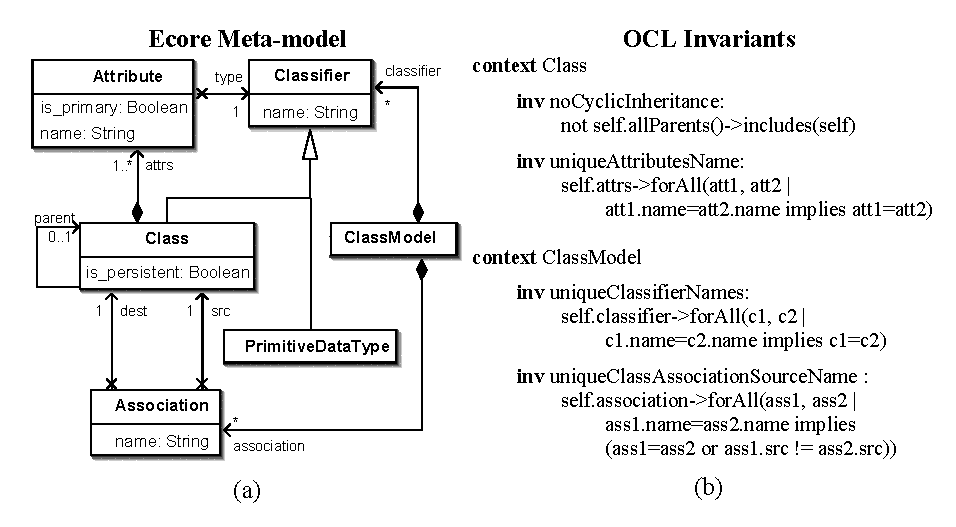
\includegraphics[scale=0.75]{./figures/classMMwithInv.eps}
\end{center}
\caption{(a) Class Diagram Subset of {\UML} {\ecore} Meta-model (b) {\OCL} constraints on the {\ecore} metamodel}
\label{fig:umlcd}

\end{figure*}

Model generation is relatively fast but performing mutation analysis is extremely time consuming. Therefore, we perform mutation analysis on {\transfo} to qualify transformation and metamodel independent strategies for model synthesis. If these strategies prove to be useful in the case of {\transfo} then we recommend the use of these strategies to guide model synthesis in the input domain of other model transformations as an initial test generation step. For instance, in our experiments, we see that generation of a 15 class simplified {\UMLCD} models takes about 20 seconds and mutation analysis of a set of 20 such models takes about 3 hours on a multi-core high-end server. Generating thousands of models for different transformations takes about 0.25\% of the time while performing mutation analysis takes most of the time. 